\documentclass[tikz, border=10pt]{standalone}
\usetikzlibrary{shapes.geometric, arrows.meta, positioning}

\begin{document}

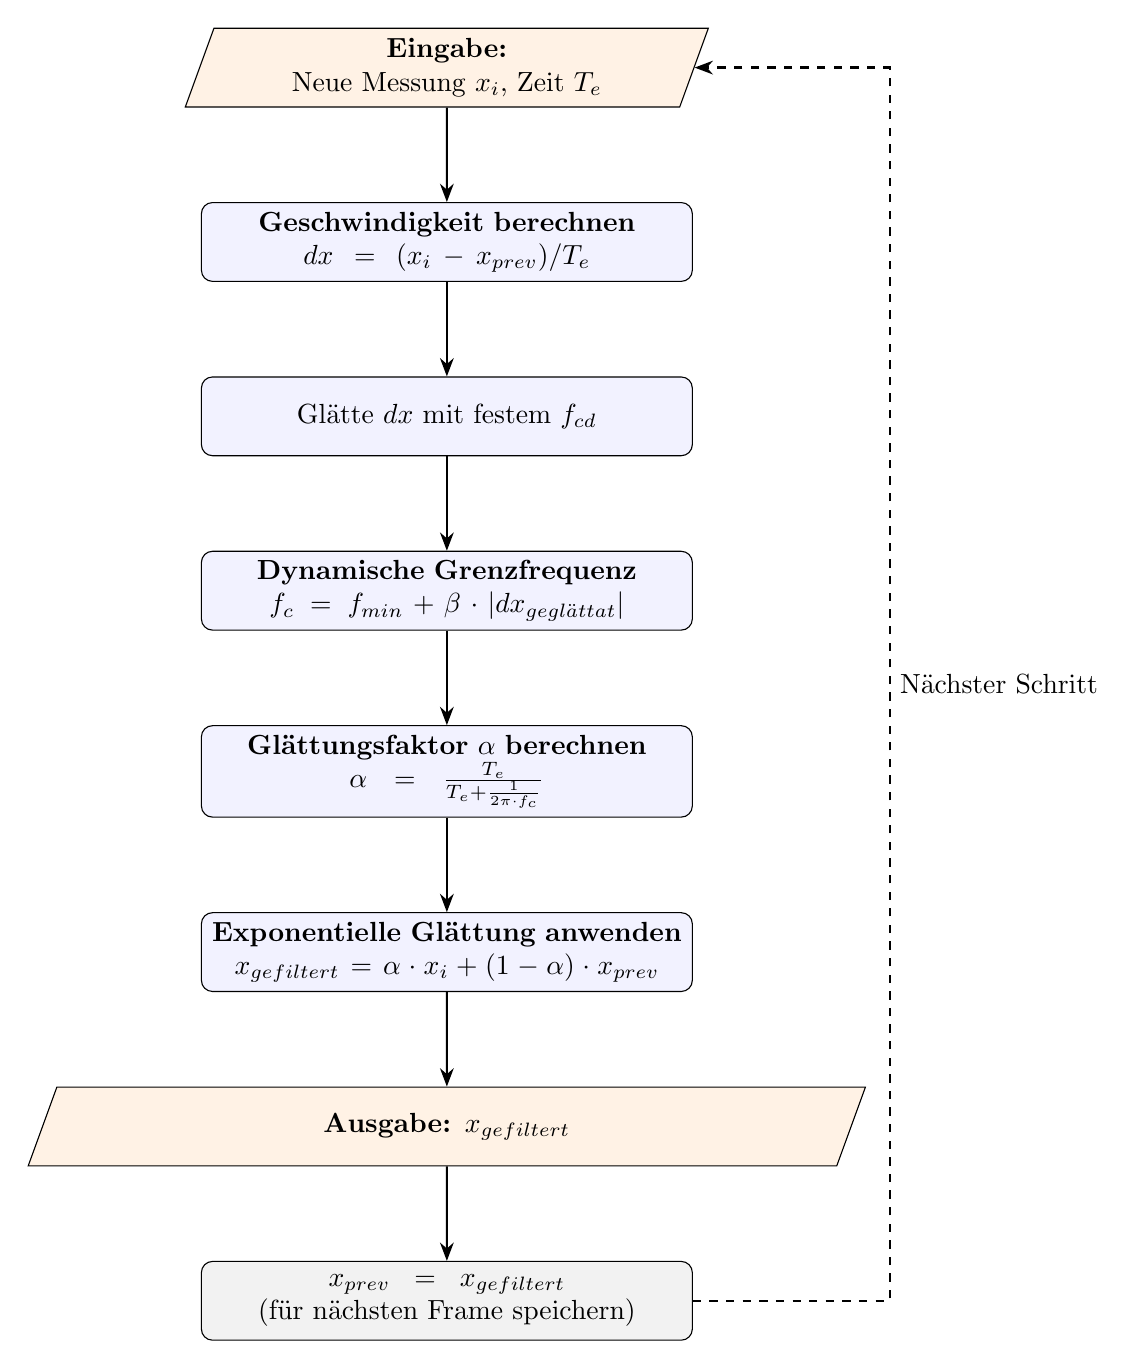
\begin{tikzpicture}[
    node distance=1.2cm,
    auto,
    block/.style={
        rectangle, 
        draw, 
        fill=blue!5, 
        text width=6cm, 
        align=center, 
        rounded corners, 
        minimum height=1cm
    },
    io/.style={
        trapezium, 
        trapezium left angle=70, 
        trapezium right angle=110, 
        draw, 
        fill=orange!10, 
        text width=5.5cm, 
        align=center, 
        minimum height=1cm
    },
    line/.style={
        draw, 
        -Stealth, 
        thick
    }
]

% Nodes
\node [io] (input) {
    \textbf{Eingabe:} \\ 
    Neue Messung $x_i$, Zeit $T_e$
};

\node [block, below=of input] (speed) {
    \textbf{Geschwindigkeit berechnen} \\
    $dx = (x_i - x_{prev}) / T_e$
};

\node [block, below=of speed] (smooth_speed) {
    Glätte $dx$ mit festem $f_{cd}$
};

\node [block, below=of smooth_speed] (cutoff) {
    \textbf{Dynamische Grenzfrequenz} \\
    $f_c = f_{min} + \beta \cdot |dx_{gegl\ddot{a}ttat}|$
};

\node [block, below=of cutoff] (alpha) {
    \textbf{Glättungsfaktor $\alpha$ berechnen} \\
    $\alpha = \frac{T_e}{T_e + \frac{1}{2\pi \cdot f_c}}$
};

\node [block, below=of alpha] (filter) {
    \textbf{Exponentielle Glättung anwenden} \\
    $x_{gefiltert} = \alpha \cdot x_i + (1 - \alpha) \cdot x_{prev}$
};

\node [io, below=of filter] (output) {
    \textbf{Ausgabe:} $x_{gefiltert}$
};

\node [block, below=of output, fill=gray!10] (update) {
    $x_{prev} = x_{gefiltert}$ \\
    (für nächsten Frame speichern)
};

% Arrows
\path [line] (input) -- (speed);
\path [line] (speed) -- (smooth_speed);
\path [line] (smooth_speed) -- (cutoff);
\path [line] (cutoff) -- (alpha);
\path [line] (alpha) -- (filter);
\path [line] (filter) -- (output);
\path [line] (output) -- (update);

% Optional: Rückführung für den nächsten Frame
\draw [line, dashed] (update.east) -- ++(2.5,0) |- (input.east) 
    node[pos=0.25, right] {Nächster Schritt};

\end{tikzpicture}

\end{document}